\documentclass{beamer}
\usepackage{etex}
\usetheme{default}
%\useinnertheme{rounded}
\usecolortheme{seagull}
\usefonttheme{structurebold}
%\usefonttheme{professionalfonts}
\usenavigationsymbolstemplate{}
%\setbeamerfont{frametitle}{family=\bfseries}

\definecolor{paprika}{rgb}{0.6,0,0.2}
\definecolor{pineglade}{rgb}{0.95,0.95,0.75}

\setbeamercolor{structure}{fg=paprika}
\setbeamercolor{block title}{fg=paprika,bg=pineglade}
\setbeamercolor{alerted text}{fg=paprika}
\setbeamercolor{block body}{bg=pineglade}
\setbeamertemplate{title page}
{%
   \begin{center}
      \begin{minipage}{0.9\textwidth}
         \begin{block}{}
            \begin{center}
              \Large{\alert{\inserttitle}}\\
              \large{\alert{\insertsubtitle}}\\
               \vspace{0.5cm}
               \large{\insertauthor}\\
               \large{\texttt{melissa.mendonca@ufsc.br}}
            \end{center}
         \end{block}
      \end{minipage}
   \end{center}
}

\usepackage[portuguese]{babel}
%\usepackage{fourier}
\usepackage[utf8]{inputenc} % To use characters such as é without typing é
\usepackage{tikz}
\usetikzlibrary{positioning}
\usetikzlibrary{arrows, decorations.markings}
% for double arrows a la chef
\tikzstyle{vecArrow} = [thick, paprika, decoration={markings,mark=at position
   1 with {\arrow[semithick,paprika]{open triangle 60}}},
   double distance=1.4pt, shorten >= 5.5pt,
   preaction = {decorate},
   postaction = {draw,line width=1.4pt, pineglade,shorten >= 4.5pt}]
% Define box and box title style
\tikzstyle{mybox} = [draw, very thick, rectangle,rounded corners, inner sep=10pt, inner ysep=20pt]
\usepackage{ctable} % provides \toprule,\bottomrule,\midrule for tables

\newcommand{\kw}[1]{\alert{\texttt{#1}}}
\newcommand{\code}[1]{{\texttt{#1}}}
\newcommand{\acode}[1]{\alert{\texttt{#1}}}
\newcommand{\codigo}[1]{\begin{center}\rm{\code{
  \begin{tabular}{r l}
  #1
  \end{tabular}
  }}\end{center}}
\newcommand{\ac}{\alert{\texttt{>>}}}
\newcommand{\file}[3]{
   \begin{center}
      \begin{tikzpicture}
         \node[mybox] (box) {
            \begin{minipage}{#1}
               #3
            \end{minipage}
         };
         \node[draw, fill=white, text=black, right=10pt, rounded corners] at (box.north west) {
            \textbf{#2}
         };
      \end{tikzpicture}
   \end{center}
}

\title{MATLAB Avançado}
\subtitle{Aula 1}
\author[M. Weber Mendonça]{Melissa Weber Mendonça}
\institute[UFSC]{\inst{1} Universidade Federal de Santa Catarina} 
\date{2014.1}

\logo{
\includegraphics[height=1.5cm]{img/brasao_UFSC.png}}

\begin{document}
%%%
% Slide 1
\begin{frame}
% Title
  \titlepage
\end{frame}
%%%%%%%%%%%%%%%%%%%%%%%%%%%%%%%%%%%%%%%%%%%%%%%%%%%%%%%%%%%%%%%%%%%%%%%%%%%%%%%%%%%%%%%%%
\begin{frame}
   \frametitle{O que é o MATLAB?}
   \begin{center}
      Linguagem computacional de alto nível e um ambiente interativo para computação numérica, visualização e programação.
      \vskip.5cm
      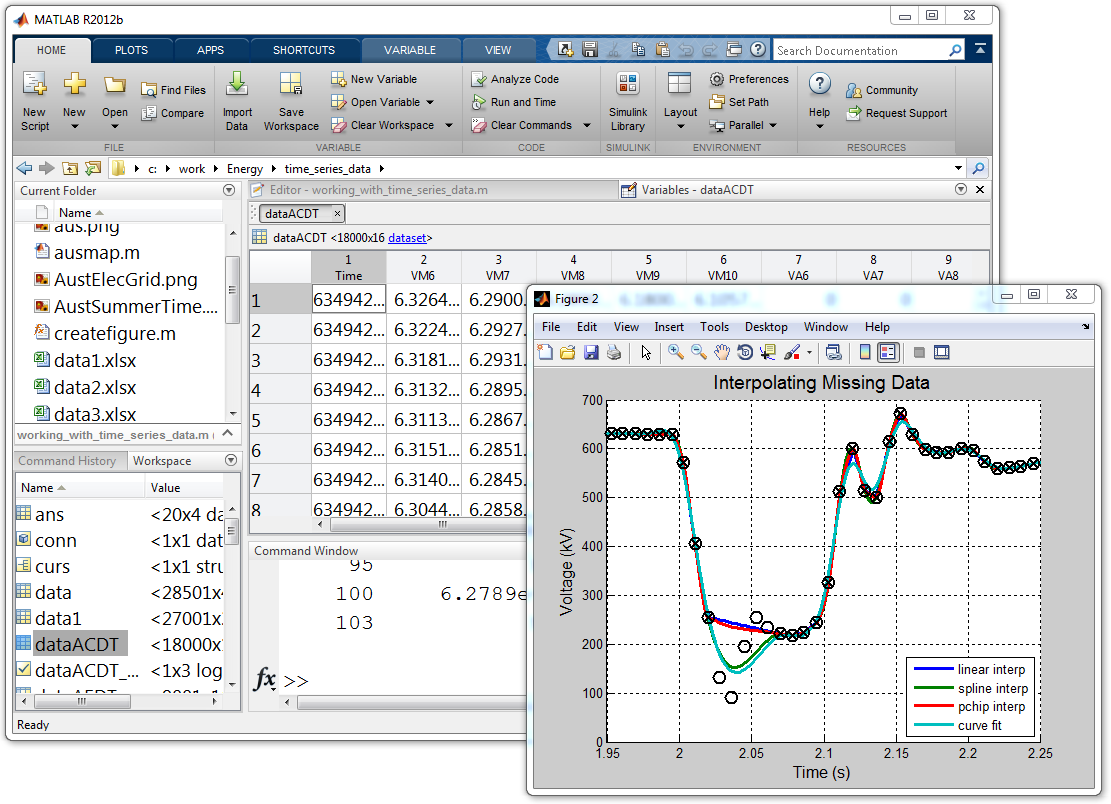
\includegraphics[width=8cm]{img/matlab.png}
   \end{center}
\end{frame}
%%%%%%%%%%%%%%%%%%%%%%%%%%%%%%%%%%%%%%%%%%%%%%%%%%%%%%%%%%%%%%%%%%%%%%%%%%%%%%%%%%%%%%%%%
\begin{frame}
  \frametitle{Console: Modo Interativo}
  \begin{center}
    \begin{tikzpicture}
      \node (console) at (0,0) {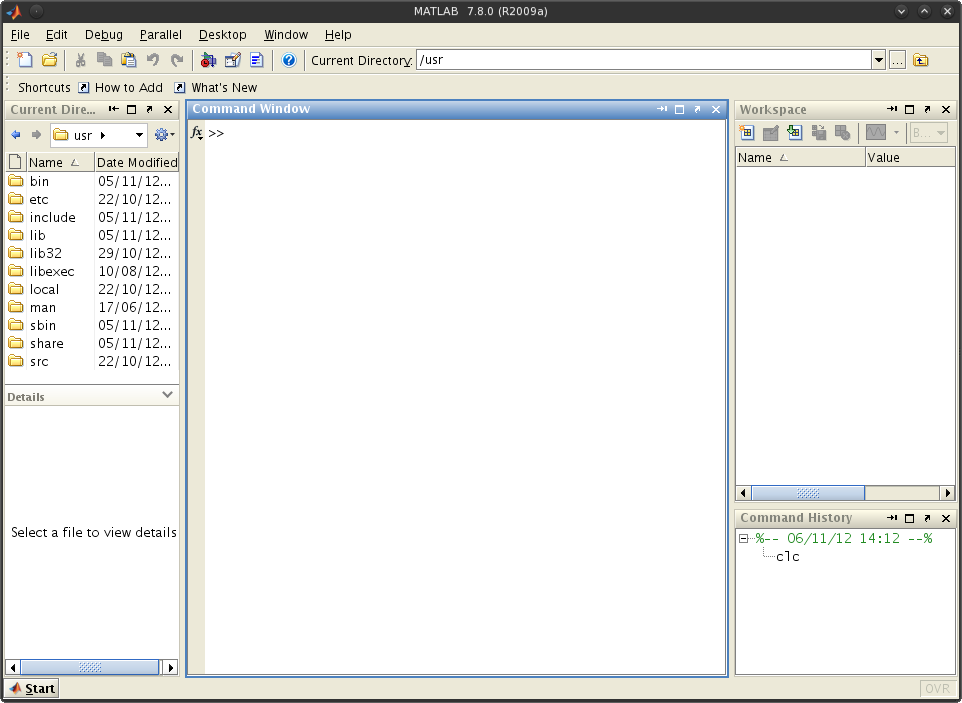
\includegraphics[width=0.6\textwidth]{img/console.png}};
      \node (consoletext) at (0,0) {\alert{Console}};
      \node[right=0.3cm of console, text width=1.7cm] (workspace) {Espaço de trabalho};
      \node[left=0.3cm of console] (files) {Arquivos};
      \node[below=0.3cm of console] (history) {Histórico};
      \node[above=0.3cm of console] (atual) {Diretório Atual};
      \draw[->, thick, paprika] (consoletext) -- (-1.5,1.2);
      \draw[->, thick] (atual) -- (0.1,2);
      \draw[->, thick] (history) -- (2.2,-1.8);
      \draw[->, thick] (workspace) -- (2.5,0);
      \draw[->, thick] (files) -- (-2.8,-0.5);
    \end{tikzpicture}
  \end{center}
\end{frame}
%%%%%%%%%%%%%%%%%%%%%%%%%%%%%%%%%%%%%%%%%%%%%%%%%%%%%%%%%%%%%%%%%%%%%%%%%%%%%%%%%%%%%%%%%
\begin{frame}
   \frametitle{Scripts}
   Os comandos podem ser entrados diretamente no \emph{console} do MATLAB, ou escritos, em sequência, dentro de um arquivo com extensão {\ttfamily{.m}} chamado \emph{script}.
   \vfill
   Sequências de trabalho possíveis:
   \begin{itemize}
      \item[1.] Escrever os comandos no console em sequência, obtendo as respostas a cada comando.
      \item[2.] Usando um script:
      \begin{itemize}
         \item[a)] Escrever os comandos em um arquivo no seu editor de texto preferido (Notepad) e salvar esse arquivo com extensão \alert{\ttfamily{.m}};
         \item[b)] Ir até a janela do console do MATLAB;
         \item[c)] Digitar o nome do arquivo em que você digitou os comandos \\\alert{sem o {\ttfamily{.m}}}.
      \end{itemize}
   \end{itemize}
\end{frame}
%%%%%%%%%%%%%%%%%%%%%%%%%%%%%%%%%%%%%%%%%%%%%%%%%%%%%%%%%%%%%%%%%%%%%%%%%%%%%%%%%%%%%%%%%
\begin{frame}
  \frametitle{}
  \begin{center}
    \alert{Estruturas de Dados e MATLAB Básico}
  \end{center}
\end{frame}
%%%%%%%%%%%%%%%%%%%%%%%%%%%%%%%%%%%%%%%%%%%%%%%%%%%%%%%%%%%%%%%%%%%%%%%%%%%%%%%%%%%%%%%%%
\begin{frame}
   \frametitle{Comandos Básicos}
   \begin{itemize}[<+->]
      \item Operações Aritméticas: \kw{+}, \kw{-}, \kw{*}, \kw{/}, \kw{\^{}}
      \item \alert{Funções} matemáticas: \kw{sin}\code{(pi)}, \kw{abs}\code{(-3)}
      \item \kw{date}
      \item \alert{\texttt{clear}} ou \alert{\texttt{clc}}
      \item \alert{\texttt{help}}
   \end{itemize}
\end{frame}
%%%%%%%%%%%%%%%%%%%%%%%%%%%%%%%%%%%%%%%%%%%%%%%%%%%%%%%%%%%%%%%%%%%%%%%%%%%%%%%%%%%%%%%%%
\begin{frame}
  \frametitle{Variáveis}
  Para atribuir um valor a uma variável no MATLAB, basta digitarmos

  \codigo{\ac & variavel = valor}

  (não é preciso declarar variáveis no MATLAB).
\end{frame}
%%%%%%%%%%%%%%%%%%%%%%%%%%%%%%%%%%%%%%%%%%%%%%%%%%%%%%%%%%%%%%%%%%%%%%%%%%%%%%%%%%%%%%%%%
\begin{frame}
  \frametitle{Introdução}
  Assim, para criar diferentes tipos de variável, usamos os seguintes comandos:
  \begin{itemize}
    \item<1-> Números (inteiros ou reais): \codigo{\ac & a = 1\\\ac & b = 3.14\\\ac & pi\\\ac & h = 1e-2}
    \item<2-> Vetores: \codigo{\ac & v = [1,2,3]\\\ac & v = [1 2 3]\\ \ac & u = [1;2;3]}
    \item<3-> Matrizes: \codigo{\ac & A = [1 2 3;4 5 6]}
    \item<4-> Texto: \codigo{\ac & texto = 'Aqui vai meu texto.'}
  \end{itemize}
\end{frame}
%%%%%%%%%%%%%%%%%%%%%%%%%%%%%%%%%%%%%%%%%%%%%%%%%%%%%%%%%%%%%%%%%%%%%%%%%%%%%%%%%%%%%%%%%
\begin{frame}
   \frametitle{Dicas}
   \begin{center}
      \begin{tikzpicture}
         \node[fill=pineglade] {
           \begin{minipage}{10cm}
               Para que o resultado \emph{não} seja mostrado ao final da operação, use \kw{;} ao final do comando.
           \end{minipage}
         };
      \end{tikzpicture}
   \end{center}
   
   Exemplo:
   
   \codigo{\ac & \acode{sin}(pi)\\
     \ac & \acode{sin}(pi);}
   
   Em um script, podemos \emph{comentar} nosso código, usando o símbolo \kw{\%}:
   
   \begin{center}
      \begin{tikzpicture}
         \node[fill=pineglade] {
           \begin{minipage}{7cm}
              \code{a = 1;}\\
              \code{\% Agora, a variável a tem valor 1.}
           \end{minipage}
         };
      \end{tikzpicture}
   \end{center}
\end{frame}
%%%%%%%%%%%%%%%%%%%%%%%%%%%%%%%%%%%%%%%%%%%%%%%%%%%%%%%%%%%%%%%%%%%%%%%%%%%%%%%%%%%%%%%%%
\begin{frame}
   \frametitle{Dicas}
   \begin{center}
      \begin{tikzpicture}
         \node[fill=pineglade] {
           \begin{minipage}{10cm}
               Para que o MATLAB imprima o valor de uma variável numérica (escalar, vetor, matriz etc), digite o nome da variável no console e pressione \emph{Enter}.
           \end{minipage}
         };
      \end{tikzpicture}
   \end{center}

   \codigo{\ac & pi}

   \begin{center}
      \begin{tikzpicture}
         \node[fill=pineglade] {
           \begin{minipage}{10cm}
               Para mostrar um texto, use o comando \acode{disp}.
           \end{minipage}
         };
      \end{tikzpicture}
   \end{center}
   
   \codigo{\ac & \kw{disp}('Oi!')}

   \begin{center}
      \begin{tikzpicture}
         \node[fill=pineglade] {
           \begin{minipage}{10cm}
              Para entrar com comandos longos em várias linhas, use \acode{...}
           \end{minipage}
         };
      \end{tikzpicture}
   \end{center}

   \codigo{\ac & soma = 1+2+3+4+5 ...\\
& \qquad +6+7+8+9+10}
\end{frame}
%%%%%%%%%%%%%%%%%%%%%%%%%%%%%%%%%%%%%%%%%%%%%%%%%%%%%%%%%%%%%%%%%%%%%%%%%%%%%%%%%%%%%%%%%
\begin{frame}
   \frametitle{MATLAB Básico: Vetores}
   \codigo{\ac & v = [1 3 5]\\
     \uncover<2->{\ac & w = [7;9;11]\\}
     \uncover<3->{\ac &  v'\\}
     \uncover<4->{\ac &  v(2)\\}
     \uncover<5->{ans =\\
       \;\; 3}\\
     \uncover<6->{\ac & \kw{length}(v)\\}
     \uncover<7->{\ac & \kw{size}(v)\\}
     \uncover<8->{\ac & \kw{size}(v,1)\\}
     \uncover<8->{\ac & \kw{size}(v,2)}}
\end{frame}
%%%%%%%%%%%%%%%%%%%%%%%%%%%%%%%%%%%%%%%%%%%%%%%%%%%%%%%%%%%%%%%%%%%%%%%%%%%%%%%%%%%%%%%%%
\begin{frame}
  \frametitle{Operações básicas}
  \begin{center}
     \begin{minipage}{0.8\textwidth}
        \begin{block}{}
           \centering{Lembre-se de respeitar as dimensões!}
        \end{block}
     \end{minipage}
  \end{center}

    \codigo{\ac & v+w-z\\
       \ac & 2*v\\
       \ac & a*w\\
       \ac & \alert{v/w}\\
       \ac & v\^{}2\\
       \ac & v.*w\\
       \ac & v./w\\
       \ac & v.\^{}2}
\end{frame}
%%%%%%%%%%%%%%%%%%%%%%%%%%%%%%%%%%%%%%%%%%%%%%%%%%%%%%%%%%%%%%%%%%%%%%%%%%%%%%%%%%%%%%%%%
\begin{frame}
   \frametitle{MATLAB Básico: Matrizes}
   \vfill
   \codigo{\ac & A = [1 2 3;4 5 6]\\
     \uncover<2->{\;\; A = \\}
     \uncover<2->{&\qquad 1 2 3\\}
     \uncover<2->{&\qquad 4 5 6\\}
     \uncover<3->{\ac & A(2,1)\\}
     \uncover<3->{\;\; ans = \\}
     \uncover<3->{\qquad 4\\}
     \uncover<4->{\ac & A'\\}
     \uncover<5->{\ac & \kw{size}(A)\\}
     \uncover<6->{\ac & \kw{size}(A,1)\\}
     \uncover<6->{\ac & \kw{size}(A,2)}}
\end{frame}
%%%%%%%%%%%%%%%%%%%%%%%%%%%%%%%%%%%%%%%%%%%%%%%%%%%%%%%%%%%%%%%%%%%%%%%%%%%%%%%%%%%%%%%%%
\begin{frame}
   \frametitle{Operações com Matrizes}
   \code{\ac\; A = [1 2;3 4]}\\
   \code{\ac\; B = [2 1;0 3]}\\
   \code{\ac\; A+B}\\
   \code{\ac\; A-B}\\
   \code{\ac\; A*B}\\
   \code{\ac\; 2*A}\\
   \code{\ac\; B/3}\\
   \code{\ac\; A'}\\
   \code{\ac\; A.*B}\\
   \code{\ac\; A./B}\\
   \code{\ac\; \alert{A/B}}
\end{frame}
%%%%%%%%%%%%%%%%%%%%%%%%%%%%%%%%%%%%%%%%%%%%%%%%%%%%%%%%%%%%%%%%%%%%%%%%%%%%%%%%%%%%%%%%%
\begin{frame}
   \frametitle{Funções básicas}
   \codigo{\ac & \acode{eye}(n)\\
     \ac & \acode{zeros}(m,n)\\
     \ac & \acode{ones}(m,n)\\
     \ac & \acode{rand}(m,n)\\
     \ac & \acode{size}(A)\\
     \ac & \acode{inv}(A)\\
     \ac & \acode{reshape}(A,m,n)}
\end{frame}
%%%%%%%%%%%%%%%%%%%%%%%%%%%%%%%%%%%%%%%%%%%%%%%%%%%%%%%%%%%%%%%%%%%%%%%%%%%%%%%%%%%%%%%%%
\begin{frame}
   \frametitle{Matrizes como vetores}
   O MATLAB permite que se acesse os elementos de uma matriz usando um índice único; nesse caso, os elementos são acessados da seguinte maneira:
   \begin{equation*}
      A(i+m(j-1)) = A(i,j),
   \end{equation*}
   com $1\leq i \leq m$, $1\leq j\leq n$, $A\in {\mathbb{R}}^{m\times n}$.
   \codigo{\ac & A(3)\\
     \ac & \kw{length}(A)}
\end{frame}
%%%%%%%%%%%%%%%%%%%%%%%%%%%%%%%%%%%%%%%%%%%%%%%%%%%%%%%%%%%%%%%%%%%%%%%%%%%%%%%%%%%%%%%%%
\begin{frame}
   \frametitle{Um texto é um vetor!}
   Um texto funciona como uma lista (vetor):
   
   \codigo{\ac & texto = 'Palavra'\\
     \ac & texto(1) = 'P'\\
     \ac & texto(2) = 'a'\\
     \ac & texto(1:2) = 'Pa'\\
     \ac & \kw{length}(texto)\\
     \ac & \kw{size}(texto)\\
     \ac & texto'}
\end{frame}
%%%%%%%%%%%%%%%%%%%%%%%%%%%%%%%%%%%%%%%%%%%%%%%%%%%%%%%%%%%%%%%%%%%%%%%%%%%%%%%%%%%%%%%%%
\begin{frame}
   \frametitle{Matrizes}
   \begin{center}
      \begin{tikzpicture}
         \node[fill=pineglade] {
           \begin{minipage}{10cm}
              \begin{center}
                 No MATLAB, tudo é matriz!
              \end{center}
           \end{minipage}
         };
      \end{tikzpicture}
   \end{center}
\end{frame}
%%%%%%%%%%%%%%%%%%%%%%%%%%%%%%%%%%%%%%%%%%%%%%%%%%%%%%%%%%%%%%%%%%%%%%%%%%%%%%%%%%%%%%%%%
\begin{frame}
   \frametitle{\emph{Slicing}}
   O MATLAB oferece uma maneira fácil de se acessar subelementos de matrizes, chamada \emph{slicing}. Nesta operação, usamos a sintaxe
   \codigo{A(linhainicial:linhafinal, colunainicial:colunafinal)}
   para acessar a submatriz determinada entre as linhas \code{linhainicial} e \code{linhafinal}, e entre as colunas \code{colunainicial} e \code{colunafinal}. Aqui, é preciso tomar cuidado para que as dimensões da matriz resultante sejam consistentes.
\end{frame}
%%%%%%%%%%%%%%%%%%%%%%%%%%%%%%%%%%%%%%%%%%%%%%%%%%%%%%%%%%%%%%%%%%%%%%%%%%%%%%%%%%%%%%%%%
\begin{frame}
   \frametitle{\emph{Slicing}}
   \codigo{\ac & A(i,j)\\
     \ac & A(i,:)\\
     \ac & A(:,j)\\
     \ac & A(:,:)\\
     \ac & A(1:2,:)\\
     \ac & A(1,2:3)\\
     \ac & A(:)}
\end{frame}
%%%%%%%%%%%%%%%%%%%%%%%%%%%%%%%%%%%%%%%%%%%%%%%%%%%%%%%%%%%%%%%%%%%%%%%%%%%%%%%%%%%%%%%%%
\begin{frame}
   \frametitle{Apagando/adicionando elementos}
   Podemos apagar elementos de matrizes (ou linhas/colunas inteiras) usando a seguinte sintaxe:
   
   \codigo{\ac & A(i,:) = []\\
     \ac & A(:,j) = []}

   Podemos também acrescentar elementos a qualquer momento:
      
   \codigo{\ac & lista = [1,3,4,5]\\
     \ac & lista = [lista 2]\\
     \ac & lista}
\end{frame}
%%%%%%%%%%%%%%%%%%%%%%%%%%%%%%%%%%%%%%%%%%%%%%%%%%%%%%%%%%%%%%%%%%%%%%%%%%%%%%%%%%%%%%%%%
\begin{frame}
   \frametitle{Dica}
   
   As operações acima também se aplicam a texto!

   \vfill

   \codigo{\ac & frase = 'Oi, como vai?'\\
     \ac & frase = [frase(1:length(frase)-1) ' você?']\\
     \ac & frase(1:2)\\
     \ac & frase = \acode{strcat}('Oi,',' como',' vai',' você?')}

   \vfill

   Atenção: \acode{strcat} não preserva os espaços em branco.
\end{frame}
%%%%%%%%%%%%%%%%%%%%%%%%%%%%%%%%%%%%%%%%%%%%%%%%%%%%%%%%%%%%%%%%%%%%%%%%%%%%%%%%%%%%%%%%%
\begin{frame}[fragile]
  \frametitle{Laços de repetição}
  Quando é necessário repetir certo comando de código várias vezes, usamos a estrutura \kw{for}:
  \begin{center}
     \begin{tikzpicture}
        \node[fill=pineglade] {
           \begin{minipage}{5cm}
\begin{verbatim}
for i = 1:3
   i
end
\end{verbatim}
           \end{minipage}
        };
     \end{tikzpicture}
  \end{center}
  Se quisermos usar um passo diferente de 1, podemos acrescentar um terceiro argumento:
  \begin{center}
     \begin{tikzpicture}
        \node[fill=pineglade] {
           \begin{minipage}{5cm}
\begin{verbatim}
for i = 3:-1:1
   i
end
\end{verbatim}
           \end{minipage}
        };
     \end{tikzpicture}
  \end{center}
\end{frame}
%%%%%%%%%%%%%%%%%%%%%%%%%%%%%%%%%%%%%%%%%%%%%%%%%%%%%%%%%%%%%%%%%%%%%%%%%%%%%%%%%%%%%%%%%
\begin{frame}[fragile]
  \frametitle{Laços de repetição (2)}
  Quando é necessário repetir certo comando de código várias vezes \alert{até que} uma certa condição seja satisfeita, usamos a estrutura \kw{while}:
  \begin{center}
     \begin{tikzpicture}
        \node[fill=pineglade] {
           \begin{minipage}{5cm}
\begin{verbatim}
i = 1;
while i < 3
   disp('Mais um.')
   i = i + 1;
end
\end{verbatim}
           \end{minipage}
        };
     \end{tikzpicture}
  \end{center}
\end{frame}
%%%%%%%%%%%%%%%%%%%%%%%%%%%%%%%%%%%%%%%%%%%%%%%%%%%%%%%%%%%%%%%%%%%%%%%%%%%%%%%%%%%%%%%%%
\begin{frame}[fragile]
 \frametitle{\acode{if} - \acode{else} - \acode{end}}
  O \acode{if} (``se'') representa uma sentença lógica condicional: 
  \vskip1cm
  \begin{center}
     \begin{tikzpicture}
        \node[fill=pineglade] (caixa) {
           \begin{minipage}{6cm}
\begin{verbatim}
if (sentença lógica)
   faça (1)
else
   faça (2) 
end 
\end{verbatim}
           \end{minipage}
        };
     \end{tikzpicture}
  \end{center}

  Em Matlab, uma sentença lógica pode ter dois valores:\\
  \begin{center} 0 (Falso) ou 1 (Verdadeiro)\end{center}
\end{frame}
%%%%%%%%%%%%%%%%%%%%%%%%%%%%%%%%%%%%%%%%%%%%%%%%%%%%%%%%%%%%%%%%%%%%%%%%%%%%%%%%%%%%%%%%%
\begin{frame}
   \frametitle{Importante}

   Atenção: ao compararmos números reais, devemos tomar cuidado com erro de arredondamento e a representação por ponto flutuante.
   
   \vskip1cm

   Exemplo: 
   \codigo{\ac & \; 3-1.1-0.9\\
      ans & =\\
      & \;\; 1.0000\\
      \ac & \; 1 == (3-1.1-0.9)\\
      ans &= \\
      & \;\; 0 \qquad \alert{(falso!)}}

\end{frame}
%%%%%%%%%%%%%%%%%%%%%%%%%%%%%%%%%%%%%%%%%%%%%%%%%%%%%%%%%%%%%%%%%%%%%%%%%%%%%%%%%%%%%%%%%
\begin{frame}
  \frametitle{Estruturas de dados Heterogêneas}

  Muitas vezes, gostaríamos de armazenar dados da seguinte forma:
  \begin{center}
     {\footnotesize{
           \begin{tabular}{l c c}
              Título & Núm. Páginas & Datas de Empréstimo e Devolução\\\toprule
              ``Álgebra Linear'' & 205 & 12/08, 15/08\\
              ``Cálculo'' & 346 & 10/09, 12/09\\
              ``Geometria'' & 123 & 04/08, 05/09\\
              ``Topologia'' & 253 & 01/08, 04/09
           \end{tabular}
        }}
  \end{center}
  Porém, estes dados são de natureza \emph{heterogênea}: misturamos texto (string), números e intervalos. Como armazenar isso em uma só tabela no MATLAB?
\end{frame}
%%%%%%%%%%%%%%%%%%%%%%%%%%%%%%%%%%%%%%%%%%%%%%%%%%%%%%%%%%%%%%%%%%%%%%%%%%%%%%%%%%%%%%%%%
\begin{frame}
   \frametitle{Estrutura \emph{Cell}}
   No MATLAB, podemos fazer o seguinte:
   \begin{itemize}
     \item[\ac] \code{tabela = \{ 'Algebra Linear', 205, [1208, 1508];}
     \item[\ac] \code{\hskip2.2cm 'Calculo', 346, [1009,1209];}
     \item[\ac] \code{\hskip2.2cm 'Geometria', 123, [0408,0509];}
     \item[\ac] \code{\hskip2.2cm 'Topologia', 253, [0108,0409] \} }
   \end{itemize}
   A célula funciona como uma matriz, mas aqui os índices são dados sempre entre chaves: \code{\{\}}.
\end{frame}
%%%%%%%%%%%%%%%%%%%%%%%%%%%%%%%%%%%%%%%%%%%%%%%%%%%%%%%%%%%%%%%%%%%%%%%%%%%%%%%%%%%%%%%%%
\begin{frame}
  \frametitle{Comandos}
  Para ver o que está armazenado na variável \code{tabela}, basta usarmos o comando
  \begin{itemize}
    \item[\ac] \acode{celldisp}\code{(tabela)}
  \end{itemize}
  Para verificar o tamanho de uma célula, usamos o comando
  \begin{itemize}
    \item[\ac] \acode{size}\code{(tabela)}
  \end{itemize}
  Para criar uma célula vazia com $m$ por $n$ elementos, usamos o comando
  \begin{itemize}
    \item[\ac] \code{tabela = \acode{cell}(m,n)}
  \end{itemize}
  Podemos também calcular a \emph{transposta} de uma célula:
  \begin{itemize}
     \item[\ac] \code{tabela'}
     \item[\ac] \code{\acode{transpose}(tabela)}
  \end{itemize}
\end{frame}
%%%%%%%%%%%%%%%%%%%%%%%%%%%%%%%%%%%%%%%%%%%%%%%%%%%%%%%%%%%%%%%%%%%%%%%%%%%%%%%%%%%%%%%%%
\begin{frame}
   \frametitle{Acessando dados dentro de uma célula}
   Existem duas maneiras de acessar elementos dentro de uma célula:
   \begin{itemize}
      \item Se usamos índices entre parênteses, estamos acessando um subconjunto da célula original.
      \item Se usamos chaves (\code{\{\}}), estamos acessando os valores no interior de cada elemento da célula.
   \end{itemize}

   Exemplo:
   \codigo{\ac & sub = tabela(1:2,1:2)\\
     \ac & tabela(2,:) = \{'MATLAB', 300, [1201, 1401]\};\\
     \ac & tabela}
\end{frame}
%%%%%%%%%%%%%%%%%%%%%%%%%%%%%%%%%%%%%%%%%%%%%%%%%%%%%%%%%%%%%%%%%%%%%%%%%%%%%%%%%%%%%%%%%
\begin{frame}
   \frametitle{Conversão de tipos}
   Note que mesmo as células que contêm valores numéricos não estão armazenadas como números. Repare nos colchetes:
   \codigo{\ac & vetor = tabela(:,2)\\
     vetor = & \\
     & \begin{tabular}{c}
        [205]\\ \relax
        [300]\\ \relax
        [123]\\ \relax
        [253]
     \end{tabular}\\
     >> & 3*vetor\\
     & \emph{Undefined function 'mtimes' for input}\\
     & \emph{ arguments of type 'cell'.}}
   
   Podemos facilmente converter esses dados para uma variável numérica usando o comano \acode{cell2mat}:
   \codigo{\ac & vetor = \acode{cell2mat}(tabela(:,2))\\
     \ac & 3*vetor}
\end{frame}
%%%%%%%%%%%%%%%%%%%%%%%%%%%%%%%%%%%%%%%%%%%%%%%%%%%%%%%%%%%%%%%%%%%%%%%%%%%%%%%%%%%%%%%%%
\begin{frame}
   \frametitle{Acessando valores}
   Para acessarmos o conteúdo de uma célula individual, usamos as chaves. Por exemplo, na nossa tabela, 
   \codigo{\ac & tabela\{1,1\}}
   é um texto com valor \code{'Algebra Linear'}, enquanto que 
   \codigo{\ac & tabela\{1,2\}}
   é um número de valor $205$.
\end{frame}
%%%%%%%%%%%%%%%%%%%%%%%%%%%%%%%%%%%%%%%%%%%%%%%%%%%%%%%%%%%%%%%%%%%%%%%%%%%%%%%%%%%%%%%%%
\begin{frame}
   \frametitle{Acessando valores - slicing}
   O resultado de um acesso simultâneo a várias células, por exemplo usando slicing, é uma \emph{lista} de valores: Note que se fizermos
   \codigo{\ac & teste = tabela\{1:3,2\}}
   a variável \code{teste} conterá apenas o primeiro resultado da operação!

   Para armazenarmos todo o resultado do acesso a estes valores da célula, podemos associar o resultado a uma lista com o mesmo número de elementos que o número de resultados do acesso:
   \codigo{\ac & [a,b,c] = tabela\{1:3,2\}}
\end{frame}
%%%%%%%%%%%%%%%%%%%%%%%%%%%%%%%%%%%%%%%%%%%%%%%%%%%%%%%%%%%%%%%%%%%%%%%%%%%%%%%%%%%%%%%%%
\begin{frame}
   \frametitle{Acessando valores - slicing}
   Se todos os elementos selecionados da célula possuirem o mesmo tipo de dados, podemos atribuir esses elementos selecionados a uma só variável. Por exemplo, neste caso todos os dados selecionados são números, e assim:
   \codigo{\ac & numpaginas = [tabela\{1:3,2\}]}

   No nosso exemplo, também temos variáveis de texto dentro da primeira coluna da célula. Podemos acessar um subconjunto do texto contido em uma das células associando os respectivos índices. Por exemplo:
   \codigo{\ac & tabela\{1,1\}(1:3)}
\end{frame}
%%%%%%%%%%%%%%%%%%%%%%%%%%%%%%%%%%%%%%%%%%%%%%%%%%%%%%%%%%%%%%%%%%%%%%%%%%%%%%%%%%%%%%%%%
\begin{frame}
   \frametitle{Outras possibilidades...}

   Célula de células:
   \begin{itemize}
      \item[\ac] \code{v = \{ \alert{\{}1, 'teste', [1;2]\alert{\}};\\
        \hskip1.2cm \alert{\{}[0,3], 12, 'nome', rand(4,4)\alert{\}} \}}
   \end{itemize}

   Neste caso, os elementos devem ser referenciados da seguinte forma:
   \begin{itemize}
      \item[\ac] \code{v\{2\}\{1\}}
   \end{itemize}
\end{frame}
%%%%%%%%%%%%%%%%%%%%%%%%%%%%%%%%%%%%%%%%%%%%%%%%%%%%%%%%%%%%%%%%%%%%%%%%%%%%%%%%%%%%%%%%%
\begin{frame}
   \frametitle{Mais comandos}
   Podemos, analogamente ao que fizemos com vetores, concatenar células:
   \begin{itemize}
      \item[\ac] \code{C1 = \{'Joao', 16\}}
      \item[\ac] \code{C2 = \{'Maria', 18; 'Ricardo', 13\}}
      \item[\ac] \code{cola = \{C1 C2\}} $\quad $ \alert{cuidado!}
      \item[\ac] \code{uniao = [C1\alert{;} C2]}
   \end{itemize}
\end{frame}
%%%%%%%%%%%%%%%%%%%%%%%%%%%%%%%%%%%%%%%%%%%%%%%%%%%%%%%%%%%%%%%%%%%%%%%%%%%%%%%%%%%%%%%%%
\end{document}
